\section{Auswertung}
\label{sec:Auswertung}
\FloatBarrier
%\begin{figure}
%  \centering
%  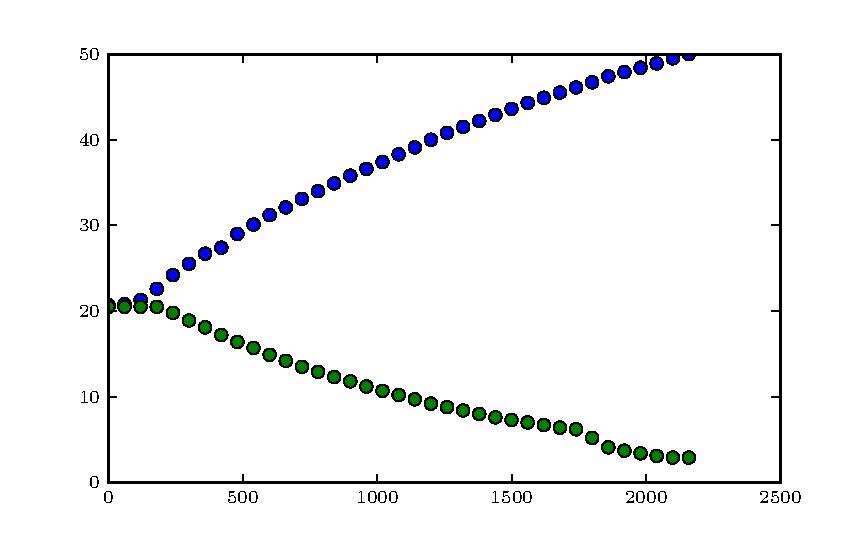
\includegraphics{plot.pdf}
%  \caption{Plot.}
%  \label{fig:plot}
%\end{figure}
\subsection{Konfiguration des Messprogramms}
\begin{figure}
  \centering
  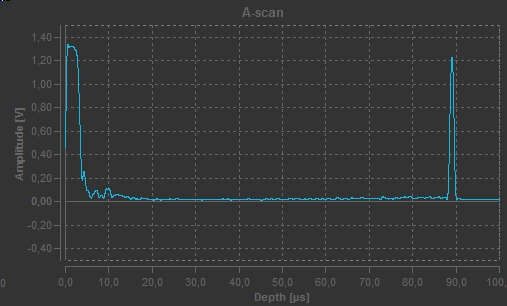
\includegraphics[width=\textwidth]{Messdaten/a.jpg}
  \caption{Amplituden-Scan zur Bestimmung der Schallgeschwindigkeit im Probenmaterial.}
  \label{fig:a1}
\end{figure}
Zur Bestimmung der Schallgeschwindigkeit im Material der vorliegenden Acrylzylinder wird die Länge eines Zylinders vermessen und die Zeitdifferenz $\Delta t$ zwischen zwei Maxima im A-Scan bestimmt.
In Abbildung \ref{fig:a1} ist der Amplituden-Scan der Messung dargestellt.
Die Zeitdifferenz zwischen den beiden Maxima bei $t_1=\SI{0.51}{\micro\second}$ und $t_2=\SI{89.20}{\micro\second}$ wird mithilfe der Cursor bestimmt zu
\begin{equation}
  \Delta t=\SI{88.69}{\micro\second} \text{.}
\end{equation}
Die Amplitudenhöhe wurde nicht vermessen, da nicht bekannt ist, wie die Verstärkung des Signals herausgerechnet werden muss.\\
Über die gemessene Länge des Acrylzylinders $s=\SI{120.5}{\milli\meter}$ ergibt sich mit Formel \eqref{eqn:laufzeit} eine Schallgeschwindigkeit von
\begin{equation}
  v_{\mathrm{Schall}}=\SI{2717.33}{\meter\per\second} \text{.}
\end{equation}
Da es zahlreiche unterschiedliche Literaturwerte für die Schallgeschwindigkeit in Acryl gibt, wird für die folgende Messung eine Schallgeschwindigkeit von $v_{\mathrm{Schall}}=\SI{2720}{\meter\per\second}$ angenommen und in das Messprogramm eingetragen.
Mit diesem Wert ist das Programm schließlich in der Lage, die Eindringtiefe der Schallwelle in das Material zu bestimmen.
Der Abstand zwischen den beiden Peaks entspricht dann der Länge des Acrylstabs.
Die durch das Programm berechnete Länge ergibt sich zu
\begin{equation}
  s=\SI{119.73}{\milli\meter} \text{.}
\end{equation}
\FloatBarrier

\subsection{Schallgeschwindigkeit über Impuls-Echo-Verfahren}
Die Zylinderlängen $s$ der mittels Impuls-Echo-Verfahrens vermessenen Zylinder samt der zugehörigen gemessenen Laufzeiten $t$ findet sich in Tabelle \ref{tab:iev}. In Abbildung \ref{fig:iev} sind die Zylinderlängen gegen die Laufzeiten aufgetragen.
Hierbei wurde der Messpunkt bei $t=\SI{82.6}{\micro\second}$ bei der Berechnung der Schallgeschwindigkeit vernachlässigt, da er deutlich vom linearen Verlauf abweicht und das Ergebnis deutlich verschlechtert.
Nach Formel \eqref{eqn:laufzeit} besteht ein linearer Zusammenhang zwischen der Zylinderlänge und der Laufzeit.
Mit python/scipy \cite{scipy} wird daher eine lineare Ausgleichsrechnung nach
\begin{equation}
  y=m\cdot x +b
\end{equation}
durchgeführt.\\
Aus dem doppelten Steigungsparameter $m$ ergibt sich die Schallgeschwindigkeit $c_\mathrm{IE}$.
\begin{gather*}
2 \cdot m=c_\mathrm{IE}=  \SI{2738(11)}{\meter\per\second} \text{,}\\
b=  \SI{11(3)}{\micro\meter} \text{.}
\end{gather*}
Der Geradenparameter $b$ ist von Null verschieden, da eine Anpassungsschicht zwischen der Sonde und dem Zylinder vorliegt. Die Ausgleichsgrade ist daher nach rechts verschoben. Die Dicke der Anpassungsschicht entspricht dabei dem Geradenparameter $b$.
\begin{table}
  \centering
  \caption{Messdaten zur Bestimmung der Schallgewschindigkeit über das Impuls-Echo-Verfahren.}
  \label{tab:iev}
  \begin{tabular}{cc}
    \toprule
    $s$/$\si{\milli\meter}$ & $t$/$\si{\micro\second}$ \\
    \midrule
    102,7 & 76,12 \\
    80,7 & 59,4 \\
    61,5 & 45,81 \\
    40,15 & 30,2 \\
    31,1 & 23,43 \\
    71,25 & 52,88 \\
    82,6 & 69,02 \\
    120,5 & 88,69 \\
    \bottomrule
  \end{tabular}
\end{table}

\begin{figure}
  \centering
  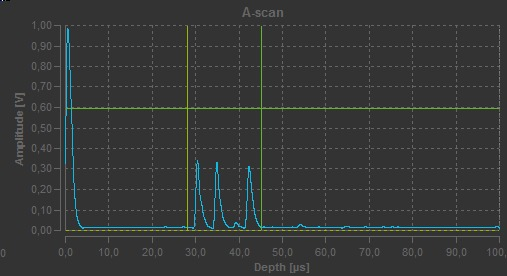
\includegraphics{Messdaten/ascan.pdf}
  \caption{Messdaten samt Ausgleichsgrade zur Bestimmung der Schallgeschwindigkeit über das Impuls-Echo-Verfahren.}
  \label{fig:iev}
\end{figure}
\FloatBarrier

\subsection{Schallgeschwindigkeit mit dem Durchschallungsverfahren}
Die Schallgeschwindigkeit wird mittels des Durschallungsverfahren erneut bestimmt.
In Tabelle \ref{tab:durchschall} finden sich die Längen der vermessenen Zylinder sowie die zugehörigen gemessenen Laufzeiten.
In Abbildung \ref{fig:durchschall} sind die Längen der Zylinder $s$ gegen die zugehörigen Laufzeiten $t$ geplottet. Mittels python/scipy \cite{scipy} wird eine lineare Ausgleichsrechnung durchgeführt.
Nach Formel \eqref{eqn:laufzeit} ergibt sich die Schallgeschwindigkeit der Durchschallmessung $c_\mathrm{Ds}$ aus dem doppelten Steigungsparameter $m$ zu:
\begin{gather*}
  2\cdot m=c_\mathrm{Ds}=  \SI{2770(40)}{\meter\per\second}\text{,}\\
  b= \SI{-53(11)}{\micro\meter}\text{.}
\end{gather*}
Der Geradenparameter $b$ ist von null verschieden. Dies entsteht durch die Dicke der Anpassungsschicht beider Sonden.
\begin{figure}
  \centering
  \includegraphics{Messdaten/d.pdf}
  \caption{Messdaten samt Ausgleichsgrade zur Bestimmung der Schallgeschwindigkeit über das Durchschallungsverfahren.}
  \label{fig:durchschall}
\end{figure}
\begin{table}
  \centering
  \caption{Messdaten zur Bestimmung der Schallgewschindigkeit über das Durchschallungsverfahren.}
  \label{tab:durchschall}
\begin{tabular}{cc}
  \toprule
$s$/$\si{\milli\meter}$ & $t$/$\si{\micro\second}$ \\
\midrule
61,5 & 24,62 \\
40,15 & 16,3 \\
39,7 & 15,91 \\
31,1 & 13,31 \\
102,7 & 38,98 \\
80,7 & 30,72 \\
\bottomrule
\end{tabular}
\end{table}
\FloatBarrier
\subsection{Bestimmung der Dämpfung mit dem Impuls-Echo-Verfahren}
Über das Impuls-Echo-Verfahren wird zudem die Dämpfungskonstante des Acryls bestimmt.
Es lässt sich Formel \eqref{eqn:dampf} umformen zu:
\begin{equation}
  \ln{\left( \frac{I(x)}{I_0}\right)}=-\alpha x \text{.}
\end{equation}
Es besteht daher ein linearer Zusammenhang zwischen der Dämpfungskonstante und dem Logarithmus des Amplitudenverhältnis.
In Tabelle \ref{tab:daempf} finden sich in die verwendeten Messdaten und in Abbildung \ref{fig:daempf} ist der Logarithmus des Amplitudenverhältnis aufgetragen gegen die Länge der Acrylstäbe aufgetragen.
Mittels einer linearer Ausgleichsrechnung mit python/scipy \cite{scipy} ergibt sich die Dämpfungskonstante aus der Steigung der Ausgleichsgrade:
\begin{gather*}
-m=\alpha=\SI{47(2)}{\per\meter} \text{,}\\
b=  \num{0.28(14)}\text{.}
\end{gather*}


\begin{table}
\centering
\caption{Messdaten zur Bestimmung der Dämpfungskonstante $\alpha$.}
\label{tab:daempf}
\begin{tabular}{cccc}
  \toprule
	$s$/$\si{\milli\meter}$ & $I_0$/$\si{\volt}$ & $I(s)$/$\si{\volt}$ & $ln\left(\frac{I(s)}{I_0}\right)$ \\
\midrule
80,7 & 0,986 & 0,018 & 4,00 \\
80,5 & 0,987 & 0,019 & 3,95 \\
61,5 & 0,987 & 0,035 & 3,34 \\
40,15 & 0,987 & 0,114 & 2,16 \\
31,1 & 0,985 & 0,189 & 1,65 \\
39,7 & 0,986 & 0,117 & 2,13 \\
\bottomrule
\end{tabular}
\end{table}

\begin{figure}
  \centering
  \includegraphics{Messdaten/amplitude.pdf}
  \caption{Messpunkte samt Ausgleichsgrade zur Bestimmung der Dämpfungskonstante $\alpha$.}
  \label{fig:daempf}
\end{figure}
\FloatBarrier
%%%%%%%%%%%%%%%%%%%%%%%%%%%%%%%%%%%%%%%%%%%%%%%%%%%%%%%%%%%%%%%%%%%%%%%%%%%%%%%%%%%%%%%%%%%%%
\subsection{Spektrale Analyse und Cepstrum}
Das aufgenommene Cepstrum ist in Abbildung \ref{fig:cepstrum} dargestellt.
\begin{figure}
  \centering
  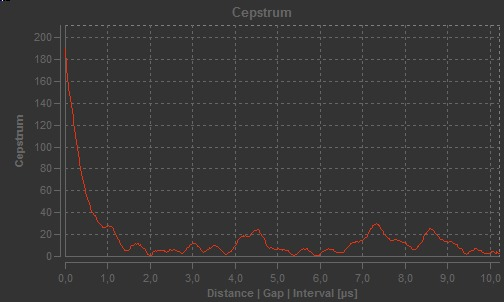
\includegraphics[width=\textwidth]{Messdaten/cepstrum.jpg}
  \caption{Cepstrum der Mehrfachreflexion.}
  \label{fig:cepstrum}
\end{figure}
Die Laufzeiten der drei zu bestimmenden Mehrfachreflexionen sind mit der Cursorfunktion
aufgenommen worden (vgl. dazu Grafik im Anhang). Um die Dicke der Acrylplatten zu berechnen, wird der Mittelwert der
bisher bestimmten Schallgeschwindigkeiten ($c_\mathrm{Ds}$ und $c_\mathrm{IE}$) verwendet. Er ergibt sich zu
\begin{equation*}
	\bar{c} = \SI{2754(16)}{\meter\per\second} \mathrm{.}
\end{equation*}
Mit Formel \eqref{eqn:laufzeit} lassen sich die zugehörigen Längen berechnen.
In Tabelle \ref{tab:cepstrum} sind die Laufzeiten mit den zugehörigen abgelaufenen Strecken
aufgetragen.
\begin{table}
\centering
	\caption{Laufzeiten der Mehrfachreflexionen bestimmt mit der Cursorfunktion und zugehörige Strecken berechnet mit Formel \eqref{eqn:laufzeit}.}
\label{tab:cepstrum}
	\begin{tabular}{ccc}
	\toprule
	Peak & $t$ / $\si{\micro\second}$ & $s$ / $\si{\milli\meter}$ \\
	\midrule
		1 & 30,41 & \num{41,6(2)} \\
		2 & 34,87 & \num{47,7(2)} \\
		3 & 42,32 & \num{57,9(2)} \\
	\bottomrule
	\end{tabular}
\end{table}
Die Dicken der Platten ergeben sich als Differenzen der abgelaufenen Strecken.
Demnach weist die erste Platte (Differenz von Peak 1 und Peak 2) eine Dicke von
\begin{equation*}
	d_1 = \SI{6,1(2)}{\milli\meter}
\end{equation*}
auf.
Analaog wird die Dicke der zweiten Platte (Differenz von Peak 2 und Peak 3)
\begin{equation*}
	d_2 = \SI{10,2(2)}{\milli\meter}
\end{equation*}
berechnet.
\begin{table}
\centering
	\caption{Messergebnisse für die Dicke der Platten mit der Schiebelehre und der Berechnung aus der Mehrfachreflexion.}
\label{tab:ceperg}
	\begin{tabular}{ccc}
	\toprule
		Platte & $d_{\mathrm{SL}}$ / $\si{\milli\meter}$ & $d_{\mathrm{CEP}}$ / $\si{\milli\meter}$ \\
	\midrule
		1 & \SI{6,1}{\milli\meter} & \SI{6,1(2)}{\milli\meter} \\
		2 & \SI{10,0}{\milli\meter} & \SI{10,2(2)}{\milli\meter} \\
	\bottomrule
	\end{tabular}
\end{table}
Die gemessenen Dicken sowie die berechneten Dicken sind in Tabelle \ref{tab:ceperg} zu finden.
Es ergibt sich also eine im Rahmen der Messgenauigkeit sehr geringe Abweichung der gemessenen
und der aus dem Ceptrum bestimmten Dicke der Platten.
\begin{figure}
  \centering
  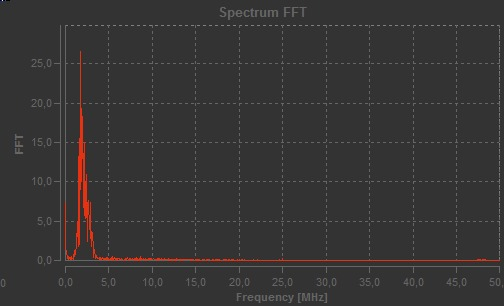
\includegraphics[width=\textwidth]{Messdaten/fft.jpg}
  \caption{Spektrum der Mehrfachreflexion.}
  \label{fig:spektrum}
\end{figure}

%%%%%%%%%%%%%%%
\FloatBarrier
\subsection{Biometrische Untersuchung eines Augenmodells}
\begin{figure}
  \centering
  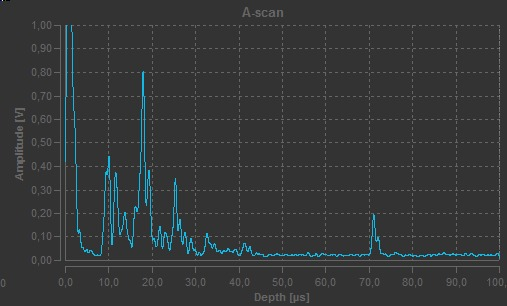
\includegraphics[width=\textwidth]{Messdaten/auge_ascan.jpg}
  \caption{A-Scan des Augenmodells.}
  \label{fig:auge_ascan}
\end{figure}
Im A-Scan des Auges (vgl. Abbildung \ref{fig:auge_ascan}) werden die fünf Peaks mit dem Cursor
zu
\begin{align*}
	t_1 &= \SI{1,15}{\micro\second} \mathrm{,} \\
	t_2 &= \SI{10,03}{\micro\second} \mathrm{,}\\
	t_3 &= \SI{17,90}{\micro\second} \mathrm{,}\\
	t_4 &= \SI{25,32}{\micro\second} \mathrm{,}\\
	t_5 &= \SI{71,02}{\micro\second}
\end{align*}
bestimmt. Die Peaks kommen durch die Reflexionen an der Oberfläche des Modells, der Iris, der
Vorder- bzw. Rückseite der Linse und der Retina zustande. Die Abstände werden unter
Berücksichtung der unterschiedlichen Schallgeschwindigkeiten in der Linse ($c_{\mathrm{L}} =
\SI{2500}{\meter\per\second}$) und in der Glaskörperflüssigkeit ($c_{\mathrm{GK}} =
\SI{1410}{\meter\per\second}$) mit Formel \eqref{eqn:laufzeit} berechnet.
Der Abstand $s_1$ wird als Abstand zwischen der Oberfläche des Modells und der Iris
definiert. Die darauffolgenden Abstände sind von der Iris aus bis zur Vorder- bzw. Rückseite
der Linse und der Retina angegeben. Es ergeben sich die Abstände:
\begin{align*}
	s_1 &= \SI{6,26}{\milli\meter} \mathrm{,} \\
	s_2 &= \SI{5,55}{\milli\meter} \mathrm{,} \\
	s_3 &= \SI{14,82}{\milli\meter} \mathrm{,} \\
	s_4 &= \SI{47,04}{\milli\meter} \mathrm{.}
\end{align*}
Außerdem muss der Maßstab 1:3 des Modells berücksichtigt werden, sodass sich die drei Abstände
\begin{align*}
	s_{\mathrm{IL}} &= \SI{1,85}{\milli\meter} \mathrm{,} \\
	s_{\mathrm{L}} &= \SI{3,09}{\milli\meter} \mathrm{,} \\
	s_{\mathrm{LR}} &= \SI{10,74}{\milli\meter}
\end{align*}
ergeben.
